44. $\cfrac{(2x^2-7x+6)(x^2+3x-10)}{(x+1)(5+4x-x^2)}\leqslant0\Leftrightarrow\cfrac{(x-2)^2(x+5)(2x-3)}{-(x+1)^2(x-5)}\leqslant0.$ Применив метод интервалов, найдём ответ: $x\in[-5;-1)\cup\left(-1;\cfrac{3}{2}
ight]\cup\{2\}\cup(5;+\infty).$
\begin{figure}[ht!]
\center{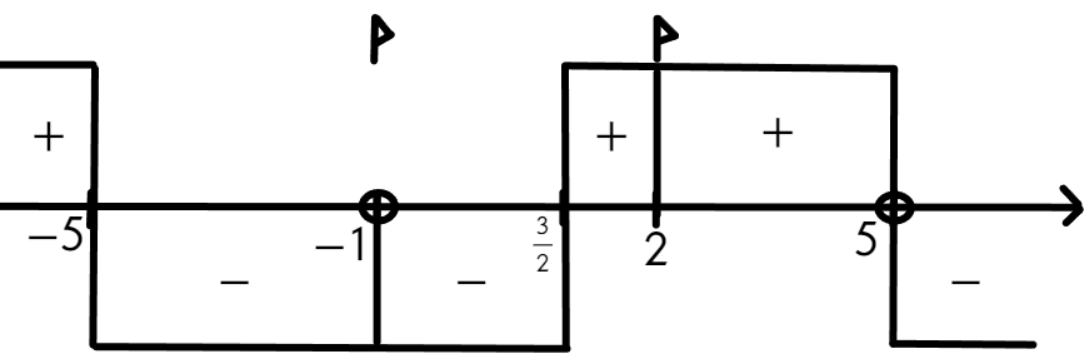
\includegraphics[scale=0.35]{ner9-44.png}}
\end{figure}
ewpage
oindent
